\documentclass[a4paper]{report}   

\usepackage[utf8]{inputenc}
\usepackage[francais]{babel}

\usepackage{graphicx}
\usepackage{hyperref}

\title{Détection d'anomalies de classification dans l'IoT via Machine Learning}
\author{Antoine Urban, Yohan Chalier}
\date{\today}

\begin{document}

\begin{titlepage}
	\centering
	\vspace{1cm}
	{\scshape\LARGE Télécom ParisTech \par}
	\vspace{1cm}
	{\scshape\Large Projet de filière SR2I \par}
	\vspace{1.5cm}
	{\huge\bfseries Détection d'anomalies de classification dans l'IoT via Machine Learning\par}
	\vspace{2cm}
	{\Large\itshape Antoine Urban, Yohan Chalier \par}
	\vfill
	encadré par\par
	Jean-Philippe \textsc{Monteuuis}\par
	Houda \textsc{Labiod}
	\vfill

% Bottom of the page
	{\large \today\par}
\end{titlepage}



\begin{abstract}
\end{abstract}

\chapter{Démarche et stratégie}

\section{Première implémentation}

\subsection{Objectif}

En premier lieu, nous souhaitions commencer par une vision globale des données et du travail à effectuer. Nous disposions d'une base de données contenant des mesures de voiture, provenant de \href{http://www.carqueryapi.com}{CarQuery}, et contenant 54808 lignes complètes. Dans cette partie, nous allons nous efforcer d'obtenir une première fonction de classification se basant sur des critères très simple : des régions de décision rectangulaires et arbitraires.

\subsection{Mise en {\oe}uvre}

Puisque l'objectif de cette étude est la détection d'anomalies dans la mesure de longueur et de largeur, nous avons extrait les deux colonnes correspondantes dans une DataFrame du module \href{http://pandas.pydata.org}{Pandas}, en Python.

Après un premier affichage des données, il est apparu que beaucoup de points apparaissaient en plusieurs fois, aussi la séparation de la base de données en points uniques et points non-uniques se révéla pertinente. Cela permit de réduire le nombre de lignes à 5026.

Manuellement, nous avons alors défini des zones simples (rectangulaires) en tant que régions de décision (Table \ref{regions_decision_manuelles_valeurs}). Ces zones ont été définies au jugé, afin d'encadrer le plus de points valides sans toutefois englober une zone de l'espace trop large.

\begin{table}[h]
\centering
\begin{tabular}{llll}
cadre & validité & intervalle de longueur & intervalle de largeur \\
\hline
vert & non-malicieux & 3 à 6,5 mètres & 1,4 à 2,4 mètres \\
gris & malicieux & 3 à 4,1 mètres & 2,05 à 2,4 mètres \\
gris & malicieux & 5,25 à 6,5 mètres & 1,4 à 1,65 mètres \\
\end{tabular}
\label{regions_decision_manuelles_valeurs}
\caption{Dimensions des régions de décision arbitraires}
\end{table}

Hors de la zone verte, et dans les deux cadres gris, nous avons alors généré aléatoirement 700 points définis comme malicieux. La figure \ref{regions_decision_manuelles_plot} représente l'affichage de tous les points décrits plus tôt ainsi que des régions de décision. Ainsi faite, notre classification possède, sur le jeu d'entraînement, une précision de 97,57\%.

\begin{figure}
\centering
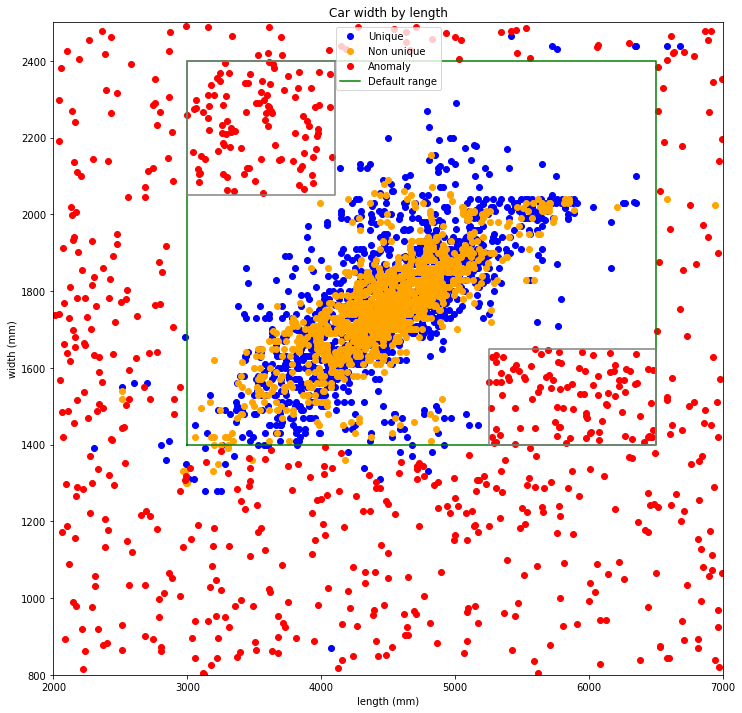
\includegraphics[width=\textwidth]{img/first_try.png}
\label{regions_decision_manuelles_plot}
\caption{Régions de décision manuelles pour des dimensions de voitures}
\end{figure}

\section{Recherche des bases de données}
\section{Environnement de travail}

\section{Méthode d'évaluation}

% \begin{thebibliography}{9}
% \end{thebibliography}

\end{document}